\chapter{伽罗瓦理论}
本章开始介绍Galois理论.如无特殊说明,本章所讨论的Galois扩张均为有限扩张.详细的参考资料可参见\cite{Patrick}\cite{ZhP}.
\section{域扩张}
\begin{definition}\index{yukuozhang@域扩张 (field extension)}\index{yukuozhang@域扩张 (field extension)!有限生成扩张 (finitely generated extension)}\index{yukuozhang@域扩张 (field extension)!单扩张 (simple extension)}\index{benyuanyuan@本原元 (primitive element)}
	设$K$和$E$均为域,如果存在域同态$\iota:K\hookrightarrow E$,则称$(E,\iota)$为$K$的\textbf{域扩张},其中$K$是域扩张的\textbf{基域},$E$为$K$的\textbf{扩域},并记为$E/K$.若存在$S\subset E$,使得$F(S)=E$,则称$E$是由$S$在$K$上生成的域.若$S$为有限集,则称该扩张为\textbf{有限生成扩张};若$S=\{x\}$,则称该扩张为\textbf{单扩张},$x$称为\textbf{本原元}.
\end{definition}
\begin{definition}\index{cishu@次数 (degree)}\index{yukuozhang@域扩张 (field extension)!平凡扩张 (trivial extension)}\index{yukuozhang@域扩张 (field extension)!二次扩张 (quadratic extension)}\index{yukuozhang@域扩张 (field extension)!有限扩张 (finite extension)}\index{yukuozhang@域扩张 (field extension)!无限扩张 (infinite extension)}\label{def:2 ext}
	每个域扩张中,扩域$E$可以看作是以基域$K$为系数域的向量空间,称扩张$E/K$的\textbf{次数}为$[E:K]=\dim_K E$.次数为1的扩张称为\textbf{平凡扩张},此时$E$与$K$同构;次数为2的扩张称为\textbf{二次扩张},可以证明二次扩张必形如$E=K(\sqrt{d})$,从而是单扩张;次数有限的扩张称为\textbf{有限扩张},否则称为\textbf{无限扩张},取向量空间的一组基可知有限扩张必为有限生成扩张.
\end{definition}
\begin{definition}\index{yukuozhang@域扩张 (field extension)!子扩张 (subextension)}\label{def:telescope}
	若存在域扩张$E/F$和$F/K$,则称$F$为\textbf{中间域},$F/K$是$E/F$的\textbf{子扩张}.此时满足关系式$	[E:K]=[E:F][F:K]$,称作\textbf{望远镜公式}.
\end{definition}
\begin{theorem}[本原元定理]\label{thm:primitive element}
	一个有限扩张$E/K$是单扩张,即存在本原元$x\in E,E=K(x)$,当且仅当$E$和$F$之间有有限个中间域.
\end{theorem}
\begin{definition}\index{yukuozhang@域扩张 (field extension)!代数扩张 (algebraic extension)}\index{yukuozhang@域扩张 (field extension)!超越扩张 (transcendental extension)}
	对于域扩张$E/K$,如果$a\in E$是$K$上非零多项式的根,则称$a$在$K$上\textbf{代数},否则称$a$在$K$上\textbf{超越}.若$E$中所有元素均在$K$上代数,则$E/K$称为\textbf{代数扩张},否则称为\textbf{超越扩张}.
\end{definition}
\begin{definition}\index{jixiaoduoxiangshi@极小多项式 (minimal polynomial)}\label{def:minimal polynomial}
	若$a$在$K$上代数,则存在唯一一个次数最小的首一多项式,称为$a$在$K$上的\textbf{极小多项式}$m_a$,则有同态映射$\pi:K[a]\to K(a)$,且$\Ker(\pi)=(m_a)$,故由同态基本定理知
	\[
	K[a]/(m_a)\cong K(a).
	\]
	由此可见以$\{1,a,a^2,\dots,a^{n-1}\}$为基的$K$-线性空间即为$K(a)$,故$[K(a):K]=\deg m_a$.故代数扩张为有限扩张,反之,$\{1,a,a^2,\dots,a^{n-1},a^n\}$必线性相关,故存在$a$的化零多项式,故有限扩张也为代数扩张.因此有限扩张无非是有限生成的代数扩张.
\end{definition}
\begin{definition}\index{yu@域 (field)!代数闭域 (algebraically closed field)}\index{daishubibao@代数闭包 (algebraic closure)}
	域$K$称为\textbf{代数闭域},若$a$在$K$上代数蕴含$a\in K$.代数扩张$E/K$ 若满足$E$为代数闭域,则称之为 $K$ 的\textbf{代数闭包},并记$E$为$\overline{K}$或$K^{\text{alg}}$.
\end{definition}
\begin{theorem}[代数基本定理]
	$\mathbb{C}$是代数闭包.
\end{theorem}
\section{正规扩张与可分扩张}
\begin{definition}\index{yu@域 (field)!分裂域 (splitting field)}
	设$E/K$为域扩张,称多项式$p\in K[x]$在$E$上\textbf{分裂},若其在$E[x]$可分解为一次因子的积.设 $\mathcal{P}$ 为 $K[x]$ 中一族非常数多项式. 若域扩张 $E/K$ 满足于
	\begin{enumerate}
		\item 每个 $p \in \mathcal{P}$ 皆在 $E$ 上分裂;
		\item 诸根 $R\coloneqq\left\{ \alpha_{p,j} : p \in \mathcal{P},\; 1 \leq j \leq \deg p \right\}$ 在 $K$ 上生成 $E$,即$E=K(R)$.
	\end{enumerate}
	则称 $E/K$ 为多项式族 $\mathcal{P}$ 的\textbf{分裂域}.
\end{definition}
\begin{proposition}
	设$f\in K[x],\deg f\geqslant1$,则$f$在$K$上的分裂域$E/K$存在且唯一,且$[E:K]\leqslant(\deg f)!$.
\end{proposition}
\begin{definition}\label{def:normal-ext}\index{yukuozhang@域扩张 (field extension)!正规扩张 (normal extension)}
	对于代数扩张 $E/K$, 以下性质等价:
	\begin{enumerate}
		\item 任一不可约多项式 $p \in K[x]$ 若在 $E$ 中有根, 则它在 $E$上分裂;
		\item 取定代数闭包 $\overline{K}/E$ 并视 $E$ 为 $\overline{K}$ 的子域, 则任意 $\iota \in \Hom_K(E, \overline{K})$ 皆满足 $\iota(E)=E$.
		\item 存在一族非常数多项式 $\mathcal{P}$ 使得 $E/K$ 是 $\mathcal{P}$ 的分裂域.
	\end{enumerate}
	满足以上任一条的代数扩张称为\textbf{正规扩张}.
\end{definition}
\begin{definition}\label{def:normal-closure}\index{zhengguibibao@正规闭包 (normal closure)}
	设 $E/K$ 为代数扩张, $\overline{K}/E$ 为选定的代数闭包. 定义 $E/K$ 的\textbf{正规闭包} $M/K$ 为 $\overline{K}|K$ 中所有含 $E/K$ 的正规子扩张之交.即
	\[
	M=\bigcap_{E\leqslant N\leqslant \overline{K}\atop N/K\text{正规}}N.
	\]
	由定义知这是包含$E$的$F$之最小正规扩张.
\end{definition}
\begin{example}\label{eg:x3-2-splitting}
	$\mathbb{Q}(\sqrt[3]{2})$的正规闭包是$\mathbb{Q}(\sqrt[3]{2},\omega)$,其中$\omega$是三次单位根.
\end{example}
\begin{definition}\index{kefenduoxiangshi@可分多项式 (separable polynomial)}\index{yukuozhang@域扩张 (field extension)!可分扩张 (separable extension)}\index{yukuozhang@域扩张 (field extension)!纯不可分扩张 (purely inseparable extension)}
	称非常数多项式$p\in K[x]$为\textbf{可分多项式},若其无重根.对于代数扩张$E/K$,若元素$a\in E$在$K$上的最小多项式为可分多项式,则称$a$在$K$上\textbf{可分}.记$E$中所有可分元素为$E_s$,此为$E/K$的中间域,则称$[E:K]_s\coloneqq[E_s:K]$为\textbf{可分次数},若$E/K$为有限扩张,则称$[E:K]_i\coloneqq[E:K]/[E_s:K]$为\textbf{不可分次数}.如果$E$中每个元素都在$K$中可分,即不可分次数为1,则称$E/K$为\textbf{可分扩张}.若可分次数为1,则称$E/K$为\textbf{纯不可分扩张}.
\end{definition}
\begin{definition}\index{kefenbibao@可分闭包 (separable closure)}
	对于$K$的代数闭包$\overline{K}$中的所有可分元素构成中间域$K^{\text{sep}}$,称为\textbf{可分闭包}.
\end{definition}
\begin{corollary}
	由本原元定理\ref{thm:primitive element},有限可分扩张必是单扩张.
\end{corollary}
\begin{definition}\label{def:perfect-field}\index{yu@域 (field)!完全域 (perfect field)}
	若域 $F$ 的所有代数扩张都是可分扩张, 也即$F[x]$中的每个不可约多项式都是可分多项式,则称 $F$ 为\textbf{完全域}.
\end{definition}
\begin{example}
	特征零域均为完全域;特征$p$域$K$是完全域当且仅当$K=K^p\coloneqq \{a^p|a\in K\}$,故有限域均为完全域.
\end{example}

\section{伽罗瓦扩张}
\begin{definition}\index{{qun@群 (group)!Galois群 (Galois group)}}\index{yu@域 (field)!不动域 (invariant field)}
	对于域扩张$E/K$,其\textbf{Galois群}定为 $\Gal(E/K) \coloneqq \Aut_K(E)$,表示保持$K$不动的$E$的自同构群.习惯用 $\Gal(E/K)$ 的群论性质来描述 $E/K$, 例如称 $E/K$ 为交换 (或循环, 可解等) 扩张, 如果 $\Gal(E/)$ 作为群是交换的 (或循环, 可解等).
	
	另一方面,若$H$为$\Aut(E)$的子群,则其\textbf{不动域}定为$\Inv(H)\coloneqq E^H$.故而有两个映射
	\begin{center}
		\begin{tabular}{rccl}
			$\Gal(E/\cdot)$&:&$E$的子域$\to\Aut(E)$的子群,&$K\mapsto \Gal(E/K)$\\
			$\Inv$&:&$\Aut(E)$的子群$\to E$的子域,&$H\mapsto\Inv(H)$\\
		\end{tabular}
	\end{center}
\end{definition}
\begin{proposition}
	设$E/K$是任意域扩张, $G=\Gal(E/K)$,则
	\begin{enumerate}
		\item $\Gal(E/\cdot)$和$\Inv$是反序的映射,即
		
		若$M_1$和$M_2$均是$E/K$的中间域,且$M_1\subset M_2$,则$\Gal(E/M_1)\geqslant\Gal(E/M_2)$;
		
		若$H_1$和$H_2$均是$G$的子群,且$H_1\leqslant H_2$,则$\Inv(H_1)\supset\Inv(H_2)$.
		\item 对于中间域$M$有$M\subset\Inv(\Gal(E/M))$;对于$G$的子群$H$有$H\leqslant\Gal(\Inv(H))$.
		\item 对于中间域$M$有$\Gal(E/M)=\Gal(E/\Inv(\Gal(E/M)))$;对于$G$的子群$H$有$\Inv(H)=\Inv(\Gal(\Inv(H)))$.
	\end{enumerate}
\end{proposition}

利用线性代数的知识我们可得以下两条有用的引理:
\begin{lemma}[Artin]
	设$H$是域$K$的自同构群的有限子群,则$[K:\Inv(H)]\leqslant|H|$.
\end{lemma}
\begin{lemma}
	设$E/K$是有限扩张,则$|\Gal(E/K)|\leqslant[E:K]$.
\end{lemma}
\begin{definition}\label{def:Galois-ext} \index{yukuozhang@域扩张 (field extension)!Galois扩张 (Galois extension)}
	设$E/K$是有限扩张,以下性质等价:
	\begin{enumerate}
		\item $E$是$K[x]$中一族可分多项式的分裂域;
		\item $E/K$是正规可分扩张;
		\item $\Gal(E/K)=[E:K]$或$[E:\Inv(H)]=|H|$,其中$H\leqslant\Gal(E/K)$;
		\item $K=\Inv(\Gal(E/K))$或$H=\Gal(E/\Inv(H))$,其中$H\leqslant\Gal(E/K)$;
		\item $E/K$是可分扩张,$F/E$是代数扩张,则$\forall\sigma\in\Gal(F/K),\sigma(E)=E$.
	\end{enumerate}
	满足以上任一条的扩张称为\textbf{(有限) Galois扩张}.
\end{definition}
\begin{definition}\index{yukuozhang@域扩张 (field extension)!复合 (compositum)}
	设 $E/K$ 为域扩张, $(E_i/K)_{i \in I}$ 为其中一族子扩张, 定义其\textbf{复合} $\bigvee_{i \in I} E_i$ 为 $E$ 中包含所有 $E_i$ 的最小域, 其元素形如有理分式
	\[
	\frac{P(x_{i_1}, \dots, x_{i_n})}{Q(x_{i_1}, \dots, x_{i_n})}, \quad Q(x_{i_1}, \dots, x_{i_n}) \neq 0,
	\]
	其中$n \geqslant 0$, $P, Q \in K[x_1, \dots, x_n]$, $i_1, \dots, i_n \in I$, $x_{i_k} \in E_{i_k}$.两个扩张的复合也写作 $E_1 E_2$.
\end{definition}
\begin{proposition}
	令$\mathcal{E}$分别为有限,代数,正规,可分, Galois,则
	\begin{enumerate}
		\item 对于扩张$E/F$,$F/K$, $E/K$是$\mathcal{E}$当且仅当$E/F$和$F/K$都是$\mathcal{E}$;(对于正规扩张例外)
		\item 扩张$E/K$的任意子扩张$F_1/K$和$F_2/K$,若$F_1/K$为$\mathcal{E}$,则$F_1F_2/F_2$也为$\mathcal{E}$.
		\item 扩张$E/K$的任意一族$\mathcal{E}$子扩张的复合和非空交仍为$\mathcal{E}$.(对于有限扩张例外,需要子扩张族有限)
	\end{enumerate}
\end{proposition}
\begin{theorem}[Galois理论基本定理]\label{thm:finite-Galois-corr}
	设$E/K$是有限Galois扩张, $G=\Gal(E/K)$,则
	\begin{enumerate}
		\item $\Gal(E/\cdot)$和$\Inv$是\textbf{互逆的}反序的映射.
		\item $G$的子群是共轭的当且仅当它们的不动域是共轭的,是正规的当且仅当其不动域是$K$的正规扩张.
		\item 设$F$为中间域,则有$\Gal(E/K)/\Gal(E/F)\cong\Gal(F/K)$.
	\end{enumerate}
\end{theorem}

Galois理论基本定理的作用是将域扩张的中间域结构,转化为特定群的子群来描述.将难以用直接的方法刻画的中间域,和可以用群论中的成熟方法刻画的有限群子群对应起来.下面介绍一个经典的例子.

\begin{example}
	重拾例 \ref{eg:x3-2-splitting} 中 $x^3-2 \in \mathbb{Q}[x]$ 的分裂域 $\mathbb{Q}(\sqrt[3]{2}, \omega)$, 注意到 $\omega$ 在 $\mathbb{Q}$ 上的极小多项式为 $x^2+x+1$. 绘制域图:
	\[\begin{tikzcd}[column sep=small]
		{} & \mathbb{Q}(\sqrt[3]{2}, \omega) \arrow[dash, d, "\text{Galois}"] \arrow[dash, ld, "\text{Galois}"'] \\
		\mathbb{Q}(\sqrt[3]{2}) \arrow[dash, rd, "\text{次数} = 3"'] & \mathbb{Q}(\omega) \arrow[dash, d, "{\text{Galois},\text{次数} = 2}"] \\
		& \mathbb{Q}
	\end{tikzcd}\]
	因为 $[\mathbb{Q}(\sqrt[3]{2}, \omega): \mathbb{Q}(\omega)] \leq 3$, 而 $2 = [\mathbb{Q}(\omega) : \mathbb{Q}]$ 和 $3 = [\mathbb{Q}(\sqrt[3]{2}) : \mathbb{Q}]$ 都得整除 $[\mathbb{Q}(\sqrt[3]{2}, \omega): \mathbb{Q}]$, 唯一的可能是 $[\mathbb{Q}(\sqrt[3]{2}, \omega): \mathbb{Q}] = 6$. 因之 $G := \Gal(\mathbb{Q}(\sqrt[3]{2},\omega)|\mathbb{Q})$ 是 $6$ 阶群. 任意 $\sigma \in G$ 的作用方式为 $\omega \mapsto \omega^{\pm 1}$, $\sqrt[3]{2} \mapsto \omega^k \sqrt[3]{2}$ ($k=0,1,2$), 并且 $\sigma$ 完全由 $(\pm, k)$ 确定, 至多有 $6$ 种选取, 于是每组 $(\pm,k)$ 都能在 $G$ 中实现.
	
	一般来说, 可分多项式的分裂域 的 Galois 群能嵌入为根集的对称群; 既然 $|G|=6=3!$, 现在可以等同 $G$ 与根集 $\{ \sqrt[3]{2}, \omega\sqrt[3]{2}, \omega^2\sqrt[3]{2} \}$ 上的对称群 $\mathfrak{S}_3$. 列举子群并考量这些子群所固定的元素, 应用定理 \ref{thm:finite-Galois-corr} 立得反序对应:
	\[\begin{tikzpicture}
		[baseline = (current bounding box.center),
		every node/.style={ },
		every edge/.style={draw},
		normaledge/.style={ sloped, edge node={node[fill=white, outer sep=0.2mm, inner sep=0mm] {$\lhd$}} }
		]
		\begin{scope}
			\node (G) at (0, 3) {$\mathfrak{S}_3$};
			\node (extra) at (0.8,3) {$G$};
			\draw (G) edge[draw=none, edge node={node {$\eqqcolon$}}] (extra);
			\node (A) at (-1, 2) {$\mathfrak{A}_3$};
			\node (H1) at (-2,1.5) {$\langle(1 2)\rangle$};
			\node (H2) at (0,1.5) {$\langle(2 3)\rangle$};
			\node (H3) at (1.5,1.5) {$\langle(1 3)\rangle$};
			\node (E) at (0, 0) {$\{1\}$};
		\end{scope}
		\draw (G) edge[normaledge] (A);
		\draw (G) edge[bend right=30] (H1);  \draw (G) edge (H2);  \draw (G) edge[sloped, edge label={$\supset$}] (H3);
		\foreach \x in {A, H1, H2, H3}
		\draw (\x) edge (E);
	\end{tikzpicture} 
	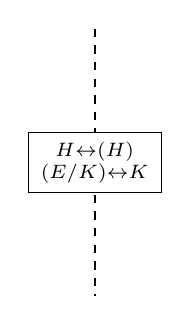
\begin{tikzpicture}[baseline= (current bounding box.center)]
		\draw[thick, dashed] (0, 1.7) -- (0, -1.7);
		\node[draw, fill=white] at (0,0) {$H\leftrightarrow \Inv(H)\atop \Gal(E/K)\leftrightarrow K$};
	\end{tikzpicture}  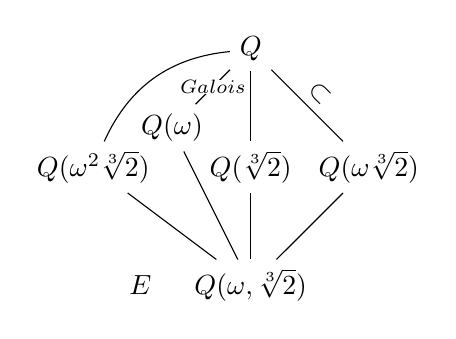
\begin{tikzpicture}
		[baseline = (current bounding box.center),
		every node/.style={ },
		every edge/.style={draw},
		normaledge/.style={edge node={node[fill=white, outer sep=0.2mm, inner sep=0mm] {\scriptsize$\text{Galois}$}} }
		]
		\begin{scope}
			\node (FG) at (0,3) {$\mathbb{Q}$};
			\node (FA) at (-1, 2) {$\mathbb{Q}(\omega)$};
			\node (FH1) at (-2, 1.5) {$\mathbb{Q}(\omega^2 \sqrt[3]{2})$};
			\node (FH2) at (0,1.5) {$\mathbb{Q}(\sqrt[3]{2})$};
			\node (FH3) at (1.5,1.5) {$\mathbb{Q}(\omega\sqrt[3]{2})$};
			\node (FE) at (0,0) {$\mathbb{Q}(\omega, \sqrt[3]{2})$};
			\node (extra) at (-1.4,0) {$E$};
			\draw (FE) edge[draw=none, edge node={node {$\coloneqq$}}] (extra);
		\end{scope}
		\draw (FG) edge[normaledge] (FA);
		\draw (FG) edge[bend right=30] (FH1);  \draw (FG) edge (FH2);  \draw (FG) edge[sloped, edge label={$\subset$}] (FH3);
		\foreach \x in {A, H1, H2, H3}
		\draw (F\x) edge (FE);
	\end{tikzpicture}\]
	
	对应的子群和中间域置于相同位置, 并以连线表示包含关系, 两侧的包含关系是上下颠倒的. 三个中间域 $\mathbb{Q}(\omega^k \sqrt[3]{2})$ ($k=0,1,2$) 两两共轭, 这从群论一面看应该是明显的.
\end{example}